\documentclass[runningheads,a4paper]{llncs}

\usepackage{amssymb}
\setcounter{tocdepth}{3}
\usepackage{graphicx}
\usepackage{subfigure}

\usepackage{url}
\newcommand{\keywords}[1]{\par\addvspace\baselineskip
\noindent\keywordname\enspace\ignorespaces#1}

\begin{document}

\mainmatter  % start of an individual contribution

% first the title is needed
\title{World building: analysing the parameters for massive evolutive generation
  of coherent backstories in fiction environments} 

% a short form should be given in case it is too long for the running head
\titlerunning{World building}

% the name(s) of the author(s) follow(s) next
%
%
\author{Non A. Me%
\thanks{NoInstitute}}
%
\authorrunning{Me, N}
% (feature abused for this document to repeat the title also on left hand pages)

% the affiliations are given next; don't give your e-mail address
% unless you accept that it will be published
\institute{No Institute}

%
% NB: a more complex sample for affiliations and the mapping to the
% corresponding authors can be found in the file "llncs.dem"
% (search for the string "\mainmatter" where a contribution starts).
% "llncs.dem" accompanies the document class "llncs.cls".
%

\maketitle


\begin{abstract}
Generating fictional worlds according to some specific requisites
presents the problem that it is impossible to know in advance the optimum for the
particular fitness function designed at the same time it creates a
vast search space for the evolutionary algorithm parameters that it
needs. In this paper our objective is to find a methodology for finding the
best parameters of the evolutionary algorithm in the design of
fictional worlds. This evolutionary design includes running, to
completion, a world represented as a chromosome and assigning a fitness to it, so it is a problem
with a very complex fitness landscape. That is why, in order to
optimize resources given to evolution and also have some guarantee
that the final result will be close to optimal, we systematically
study the values of different parameters to try and find a set of
rules that will, once you have the fitness function, help you set a
reduced range of values or even a single value that will, with a
reduced computation budget, help you find an optimal world.

\keywords{Games, Plot, evolutionary algorithms, content generation, literature}
\end{abstract}

\section{Introduction}

In the very competitive cultural industry, writers rack their minds in
order to generate interesting fictional worlds, mainly for the
creation of richer environments in modern videogames. In order to make
generation of these fictional worlds and the stories within them truly efficient and massive,
several methods have been proposed \cite{garcia14my,nairat:evolution}. One of them, called MADE
\cite{garcia14my} finds ``interesting'' character stories by running
an evolutionary algorithm that optimizes a fitness function designed
from the archetypes that best describe the world the client wants.

MADE works as follows: every individual in an evolutionary algorithm
is described by a chromosome that represents one (or several kinds of)
finite state automaton that are set to live in a simulated
environment. The evolutionary algorithm was run with standard
parameters and {\em sensible} default values were given to several
non-evolutionary parameters such as the number of profiles needed to
obtain the desired result and or the size of the simulated
world. There was no attempt to optimize these parameters, since the
main intention seemed to be to have a prototype that allowed the
authors to have an acid test of their proposed approach.

That paper hinted at the fact that parameters such as the number of
{\em profiles} (different kind of finite state automaton present in
the world) had a big influence on the outcome, to the point of making
it possible or not. However, other parameters such as the number of
simulated days the world is running might also have some influence.

In this paper we will use that open source simulator and look at it
from the evolutionary point of view so that we can check what kind of
influence they have in the outcome. We will do a experimental setup
that will test different parameters, and eventually find a series of
rules that will help the users of that framework to set the best
values for their simulation. 

The rest of the paper is organized as follows. Coming up next, we
present the state of the art in parameter setting of simulated
worlds. Next we will present the experimental setup we follow in this
article, whose results will be shown in Section \ref{sec:res}. Finally, we will
present the conclusions reached in this paper.

\section{State of the Art}
%TODO @raiben (aunque he empezado yo, la vamos a hacer de forma histórica empezando por lo antiguo, diciendo qué cosas tomamos de cada uno y terminando en MADE y cómo lo mejoramos) No olvides citar a nairat:evolution y explicar lo que dijo Morrell
 

Literary content generation has been studied since the XXs ... First papers ...  Morrell \cite{MorrellFiction06} defines those elements as ...

Then...

A methodology to systematise the generation of backstories in massive worlds 
using GAs was presented by García-Ortega et al. in \cite{garcia14my}. In that
paper, the steps to define the elements of a complex world, and how to optimise 
their character's behaviour using GAs to extract information, were presented. 
Also, that work included a preliminary analysis of one parameter: the number of
profiles. Results in that paper shown that this parameter have significant 
difference in the archetype-based fitness attained. The open-source simulator 
MADE, used here, was also presented in that work. However, the rest of 
parameters that conform the fictional setting (defined in 
\cite{MorrellFiction06}) were set as ad-hoc parameters. In this paper, we want 
to extend that study testing the rest of the parameters that model a story: the
time, the world, the OBJECT and the characters.

\section{Methodology and experimental setup} %Issue #12
\label{sec:met}

In this section we will show how to systematize the different steps
of the proposed method to generate a fictional world. Initially, the
fitness should be decided with the desired behaviour of the
agents that populate the world (for example, a given quantity of some
archetype) in mind. To enable the generation of different
personalities different number of ``profiles'' could be required. This concept,
presented in \cite{garcia14my}, describes the different sets of behaviour
parameters of the agents in the world (the number of different
FSMs). Therefore, a world with three profiles is composed by three different
types of agents. However, and as demonstrated in \cite{garcia14my}, the
number of profiles could be different of the number of desired
archetypes, as some archetypes can be shared, or on the contrary, impossible to obtain with a certain number of profiles.
That is the reason we will add this parameter in the experimental setup. % Is this the main point of the paper? Wasn't this proved
            % in the alife paper? - JJ FERGU: you are right, changed

Then, the characteristics of this world are also decided taking into account the expected... For example, adding enough days to allow the archetypes generation. Finally, the interesting plot points are extracted from the log using... % !!! Explain this!!! - JJ TODO @raiben

In this work, we propose three scenarios:
\begin{itemize}
\item Scenario A: The Villains. This scenario only requires one type of archetype: The ``villain''. This % don't leave me this way!!! FERGU: this has to be written by @raiben (TODO @raiben)
\item Scenario B: The Hero. As in the classic stories, when a villain appears, a hero must rise. The ``hero'' archetype depend on the existence of a ``villain'' archetype. This scenario tries to generate worlds formed by archetypes that depend of anothers.
\item Scenario C: The Shakespearian story. As many of the great stories of The Bard, this world requires the existence of different and interdependent archetypes: The ``hero'' and ``villain'' are completed with the ``obstacle'' (QUE HACE QUE), the  ``mentor'' (QUE HACE QUE) and the ``avenger'' (this archetype does not depend on the others).

\end{itemize}

\subsection{Designing a fitness function}

% Una vez más, no usáis ninguna metodología para hacer esto. Es un poco ``Se me ha ocurrido hacerlo así''. - JJ FERGU: ¿como podemos hacerlo?

The first step requires to develop a fitness function that takes into
account the quantity of the desired archetypes. This fitness function
should enable the existence of diversity in the desired
archetypes: that is, it is better that the world has 25\% of
``villains'' and 25\% of ``heroes'' than 50\% of ``villains'' and no
``heroes''. Thus, we propose the following fitness function: 

\begin{equation}
F_A= {\sum _{i=1}^{A} {\log \left( 1+10p_{i}\right) } \over {\log 1}}
\end{equation}

where $A$ is the number of desired archetypes, and $a_{i}$ is the
percentage (from 0 to 1) of a specific archetype in the world. % Why
                                % logs and all the rest? - JJ FERGU: TODO @raiben hablar de arquetipos y completar lo de abajo

In this paper, three fitness functions will be studied a different one
for every previously explained scenarios:
\begin{itemize}
\item Function 1 ($F_1$): for the scenario A . This function requires the maximization of the ``villain'' archetype, trying to maximise the number of villains in the world. 
\item Function 2 ($F_2$): for the scenario B. In this, case, the ``hero'' archetype... and villain ()
\item Function 3 ($F_5$): for the scenario C... This function requires 5 different archetypes. These archetypes have some type of interdependence. hero villano obstaculo mentor y vengativo %(este no deènde de nadie)
\end{itemize}

\subsection{Individual representation}


An individual in the EA is a vector of parameters that model the behaviour of {\em all} the agents in the world (keep in mind that an individual of the EA is not equal to an agent in the world). These parameters have been presented in \cite{garcia14my}, and they define the transitions and states of a Finite State Machine that model the agent's behaviour. 

This vector of parameters is composed by several {\em profiles}. The number of profiles has a direct relation with the desired fitness function. It is expected that functions with only one kind of archetype (such as F1) only would require one profile (or set of parameters). However, as explained in \cite{garcia14my}, to allow the existence of different personalities in the world, different sets of personalities (or profiles) can be evolved at the same time. Therefore, the number of profiles affect the generated fitness, as the chromosome will be larger. 
% Chromo what? FERGU: arreglado


\subsection{System optimization}


Once the fitness function has been decided, several parameters related with the world and the GA will be studied. As explained before, the parameters that define a literary story are the time, the world, the characters and the object. In this paper, we use the elements defined in MADE: number of days (time), a grid (world), food (object) and rats (characters).

%TODO rubén, que no se te olvide hablar de esto en la intro como viene en el issue y que esté relacionado con lo que pongo aquí. Por ejemplo, llamar al "object" de otra forma

Different parameter values for each element will be studied to clarify their influence in the literary world generation. First, it is expected that the number of days will have a significant impact, as larger values will allow the generation of more backstories. The set of days to study will be 64, 128 and 256. The world size (size of the grid in this paper: 5x5, 10x10 or 20x20) can also influence in the execution of the story, as larger worlds could make the agents spent more time exploring before an event occurs. The food, or the element that condition the actions (attack, share and defend among others), also could have enough effect in the story generation: lower quantities of food may increase the attacks, creating more aggressive agents, and larger quantities may generate more generous agents. Different proportions of food depending of the world size will be studied (food placed in 1/2, 1/4 and 1/8 of the size of the map).

Also, it is expected that the existence of different personalities (or number of profiles) in the world will have a significant effect in the runs, specially in functions that require more than one archetype. We will compare the usage of 1, 2, 4 and 8 profiles in each scenario. As the usage of different number of profiles generate different
individual sizes, and therefore different convergence times, the stop
condition will be established depending of the best fitness (30 generations without improvement), to do a fair comparison.

Finally, the parameters of the GA also affect the values of the
obtained world. In this paper, we study the population size, a parameter that has big effect in the execution of this kind of algorithms \cite{}, comparing populations of 64, 128 and 256 individuals. %TODO citar a un paper de tamaños de poblacion

Table \ref{tab:parameters} summarizes all the configuration parameters that will be compared (with their acronyms used in this paper), and the rest of the (fixed) parameters of the algorithm. The fixed values of the parameters of the GA have been usually described by other authors as...

The rest of the parameters of the MADE environment, such as the initial number of agents in the world, and the agent's parameters (such as the lifespan) are described in \cite{garcia14my}. In this paper we will use the default values presented in that work.

\begin{table*}
\begin{center}
\begin{tabular}{|c|c|}
\hline
{\em Parameter} & {\em Values} \\\hline \hline
\multicolumn{2}{|c|}{Parameters under study} \\ \hline \hline
Number of profiles (P) & 1, 2, 4 and 8 \\\hline
Number of virtual days (D) &  64, 128 and 256 \\ \hline
World dimension (W) &  5x5, 10x10 and 20x20 \\ \hline
Food (F) & 1/2, 1/4, 1/8 \\ \hline
GA population size & 64, 128 and 256 \\ \hline
\multicolumn{2}{|c|}{Fixed parameters} \\ \hline \hline
Mutation probability & 1/12 per gene \\ \hline
Parent pool size & Same as pool size \\ \hline
Selection method & Binary tournament \\ \hline 
Elite & 10\%  \\ \hline
% Cuando algo no compile lo arregláis, no lo borréis!!!! - JJ FERGU: ups, se me había pasado
Replacement method & Generational\\ \hline
Stop condition & 300 gens. or 30 gens. without improvement \\ \hline
%Stop condition? - JJ FERGU: puesta 
% Without improvemente in what? It's noisy fitness... no change in the
% best individual? - JJ
Runs per configuration & 30 \\ \hline
\end{tabular}
\caption{Parameters used in the experiments.}
\label{tab:parameters}
\end{center}
\end{table*}

%\subsection{Converting logs to stories}
% This subsection is *very* important... and not there yet. - JJ

% 12 pages is the limit.
\section{Results}
\label{sec:res}

In this paper, 9720 runs were carried out for each problem/scenario (30 times * 4 levels for \emph{P} * 2 levels for \emph{D} * 3 levels for \emph{W} * 3 levels for \emph{S} * 3 levels for \emph{F} that represent the possible combinations) to obtain the fitness for each combination.

Since the Kolmogorov-Smirnov test determines that the data we are using
does not follow a normal distribution a non-parametric test, the Kruskal–Wallis test, has been
performed.  % por
                                % favor, ¿podéis escribir esto EN
                                % INGLÉS? - JJ FERGU: esto se ha extraido de un paper de ANOVA de hace tiempo, pero he quitado la última frase

The application of Kruskal-Wallis consisted in running the EA optimization method using those parameter combinations to obtain the best fitness. 
The response variable used to perform the statistical analysis is the fitness at the end of the run. The changes in the response variable are produced when a new combination of parameters is considered. Then, the {R} \footnote{{\tt http://www.r-project.org}} tool was used to obtain the Kruskal-Wallis tables as well as the tables of means and figures for each problem.

The tables obtained by the Kruskal-Wallis analysis show for each factor the  degrees of freedom (FD), the experimental value of the statistical F (F value) and its associated p-value. If the output is smaller than 0.05, then the
effect of this factor is statistically significant at a $95\%$
confidence level (which indicates that different initial values of
this parameter lead to significant differences on the fitness).

We have obtained values lower than 0.05 for all parameters in all scenarios (generated p-values tables have been omitted due to space constraints). These results show that all the parameters considered have a significant
impact in the generation of the agents behaviour. This confirm our hypothesis that the four elements that conform a story (time, characters, OBJECT and world) have a great repercussion in the generation of stories in the simulation environment. %TODO @raiben poner el concepto del OBJECT que vamos a usar

Since a significant p-value only tells  that the effects are not all
equal (i.e., reject the null hypothesis), post-hoc tests might be used
to determine which effects or outputs are significantly different from
which other. % are we using them? - JJ FERGU: yes, abajo.

Therefore, a Kruskal-Wallis multi-comparison test has also been
performed, showing significant differences among all parameter values,
except for number of profiles (only using 1 profile has significant
difference with respect to use 2, 4 and 8), and GA population size
(64-128 and 128-256), both values (number of profiles and GA population size) in the scenarios Villain and Hero. This
can be explained because only one profile is necessary in these
scenarios (as the hero and villain archetypes are based in attacking
other rats, and therefore, can be shared by the same agent). Therefore, 
the fitness function $F_1$ and $F_2$ only differs in counting the archetype of an ``attacking'' rat almost twice.  % Yo no
                                % lo explicaría en términos de lo que
                                % nosotros nos imaginamos, sino en
                                % términos del propio algoritmo y su
                                % función de fitness. FERGU: lo he intentado, pero no lo tengo muy claro @raiben, escribe tú

% Deberías agruparlos por parámetro, no por escenario. No estás
% comparando diferentes parámetros de un escenario, sino diferentes
% niveles para un parámetro - JJ FERGU: tienes toda la razón, agrupado

All the results have been also plotted in order to understand better
their differences (in Figures \ref{fig:boxplotsP} to \ref{fig:boxplotsS}). At first glance, the median for D, W and F is 0 (or almost 0) for several
values. This can be explained for different reasons. First, the number of profiles has enough impact in the results (Figure \ref{fig:boxplotsS}), as it was shown previously in \cite{garcia14my}. Although no executions achieved the maximum number of generations (300), the length of the chromosome have an effect in the convergence. %FERGU: @raiben habría que hacer lo que dice JJ de estudiar qué eventos se están produciendo. El problema es que habría que lanzar todo otra vez... Pienso que tampoco sería mala idea hacer un estudio respecto al parámetro GENERATION con los Kruskal-Wallis, para ver cuando paran los EAs y justificar mejor este párrafo.

With respect to the parameter D it can be seen in Figure \ref{fig:boxplotsD} a small
amount of days (64) is not enough to allow the generation of any
archetype, as there is no time to develop a story in any of the scenarios. This can also be
related to the world dimension (Figure \ref{fig:boxplotsW}): larger worlds require more time to be
explored, so the chances of an encounter that can trig an event (for
example, a fight) is more difficult. 

Finally, the amount of food (Figure \ref{fig:boxplotsF}), the
element that makes most actions appear, also need to be low enough to
promote fightings (1/8 of the world size). 



% which is interesting
% because... - JJ FERGU: explicado todo




\begin{figure}
        \centering
        \subfigure[\scriptsize{Scenario 1: Villain}]{
                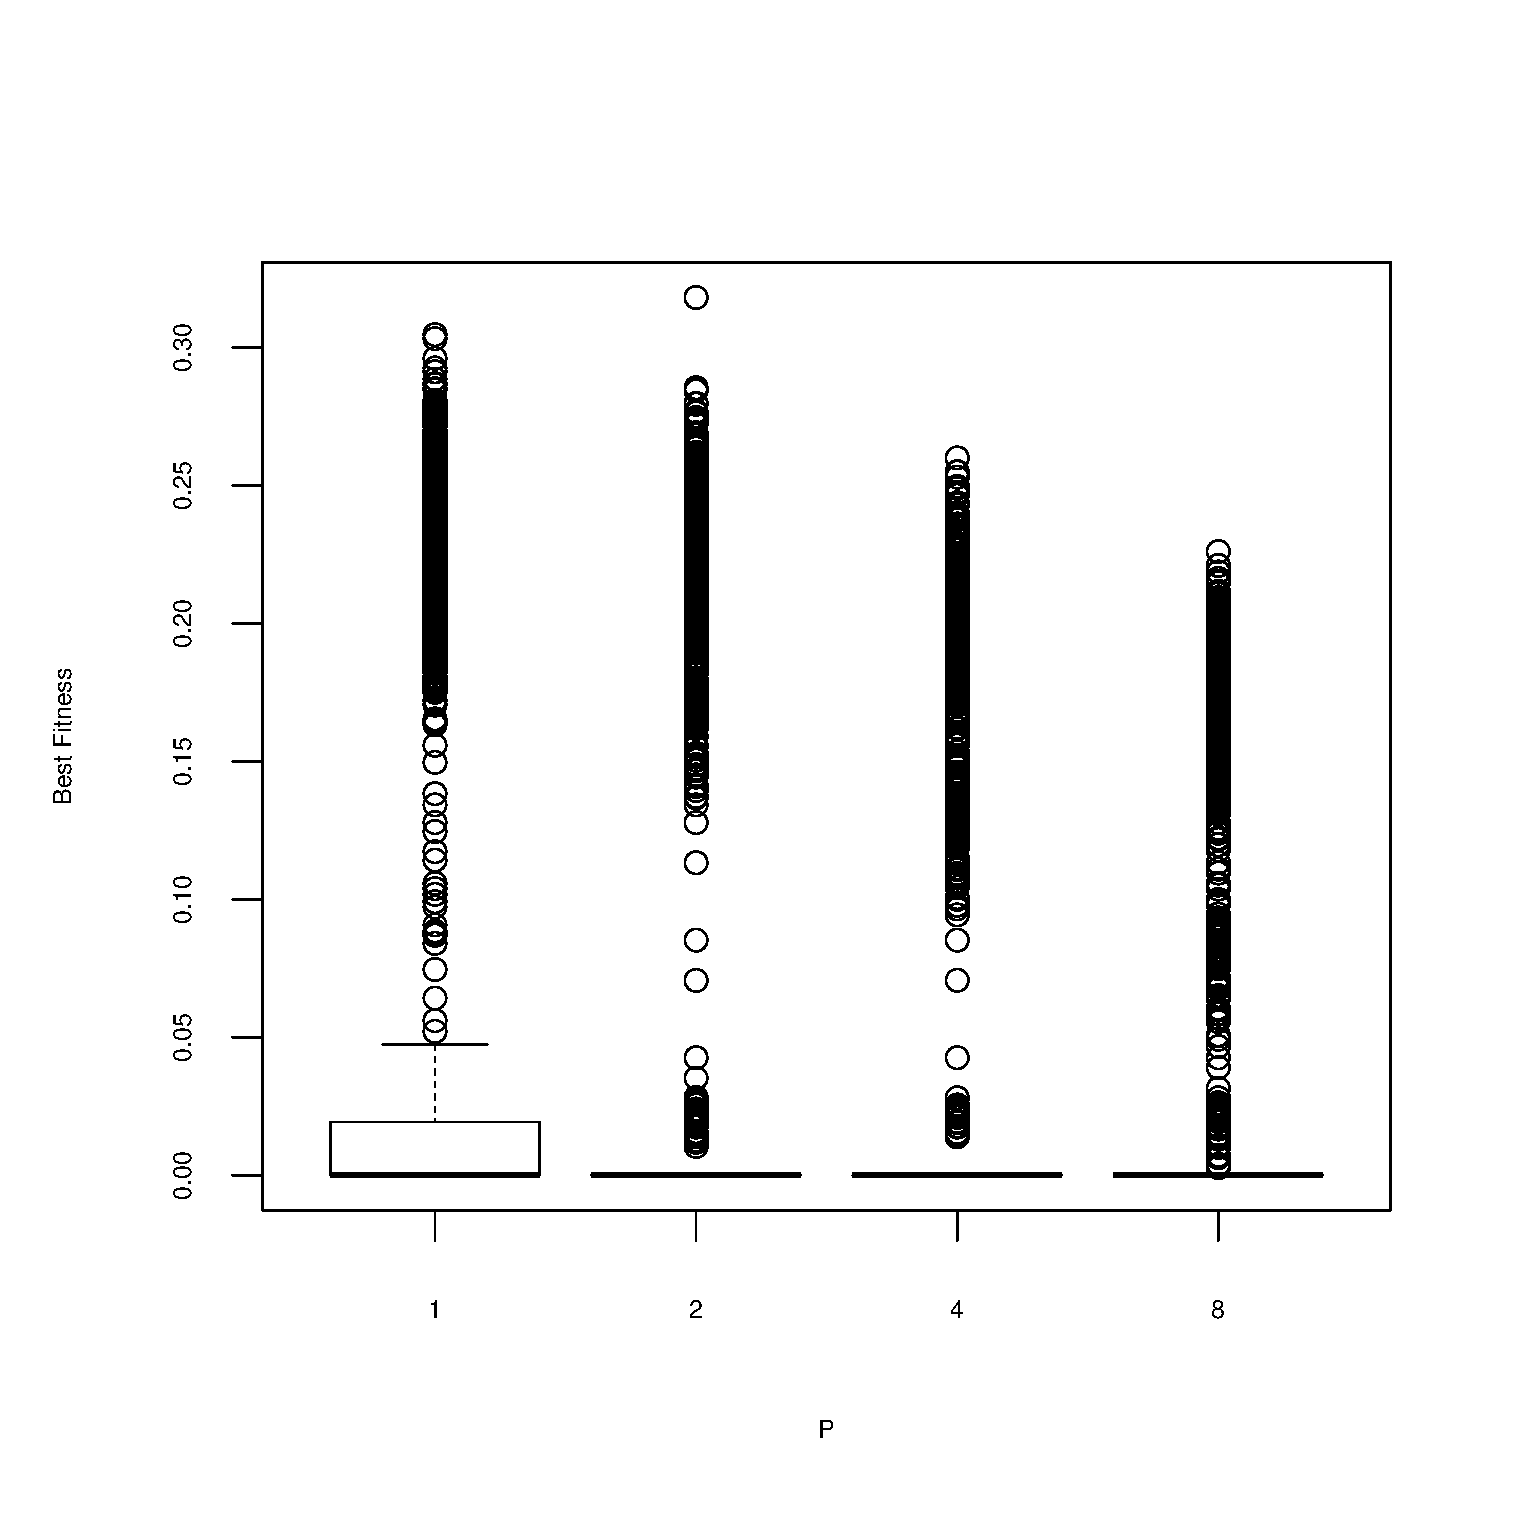
\includegraphics[width=3.7cm]{imags/boxplotz1P.eps}
                \label{fig:e1_p}
        }
        \subfigure[\scriptsize{Scenario 2: Hero}]{
                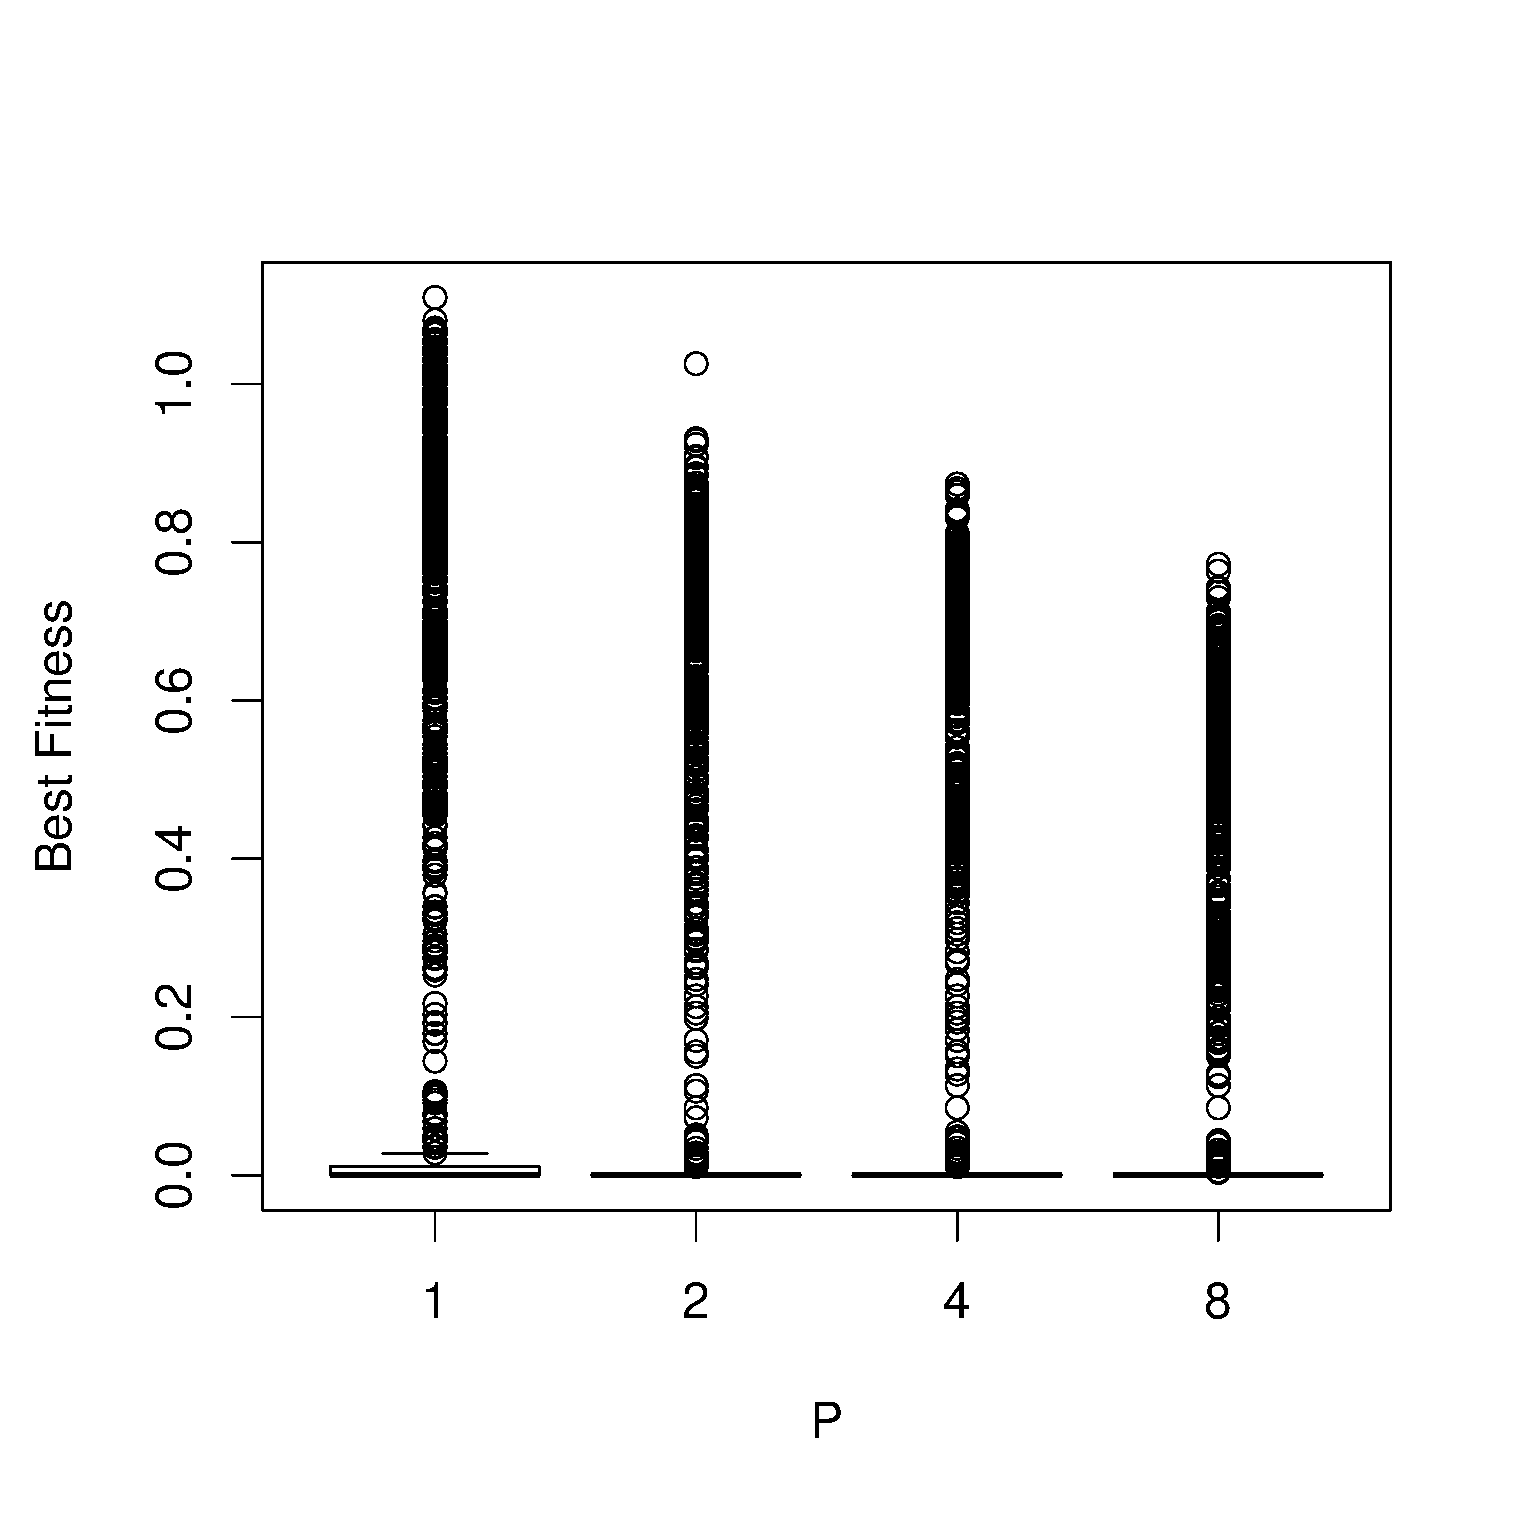
\includegraphics[width=3.7cm]{imags/boxplotz2P.eps}
                \label{fig:e2_p}
        }
        \subfigure[\scriptsize{Scenario 3: Shakespearian}]{
                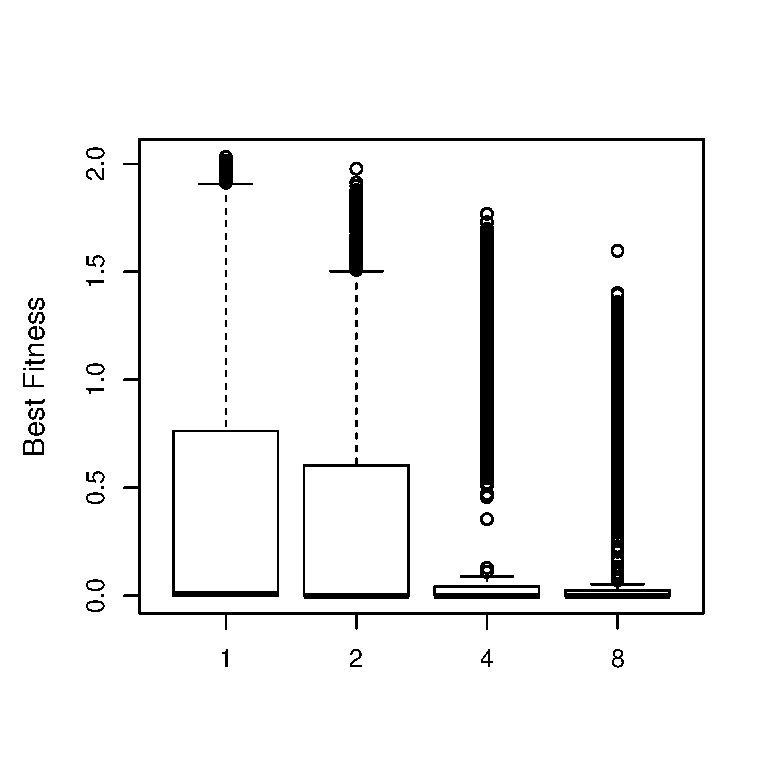
\includegraphics[width=3.7cm]{imags/boxplotz5P.eps}
                \label{fig:e3_p}
        }  
        \caption{Boxplots for parameter P (number of profiles)}\label{fig:boxplotsP}
\end{figure}



\begin{figure}
        \centering
        \subfigure[\scriptsize{Scenario 1: Villain}]{
                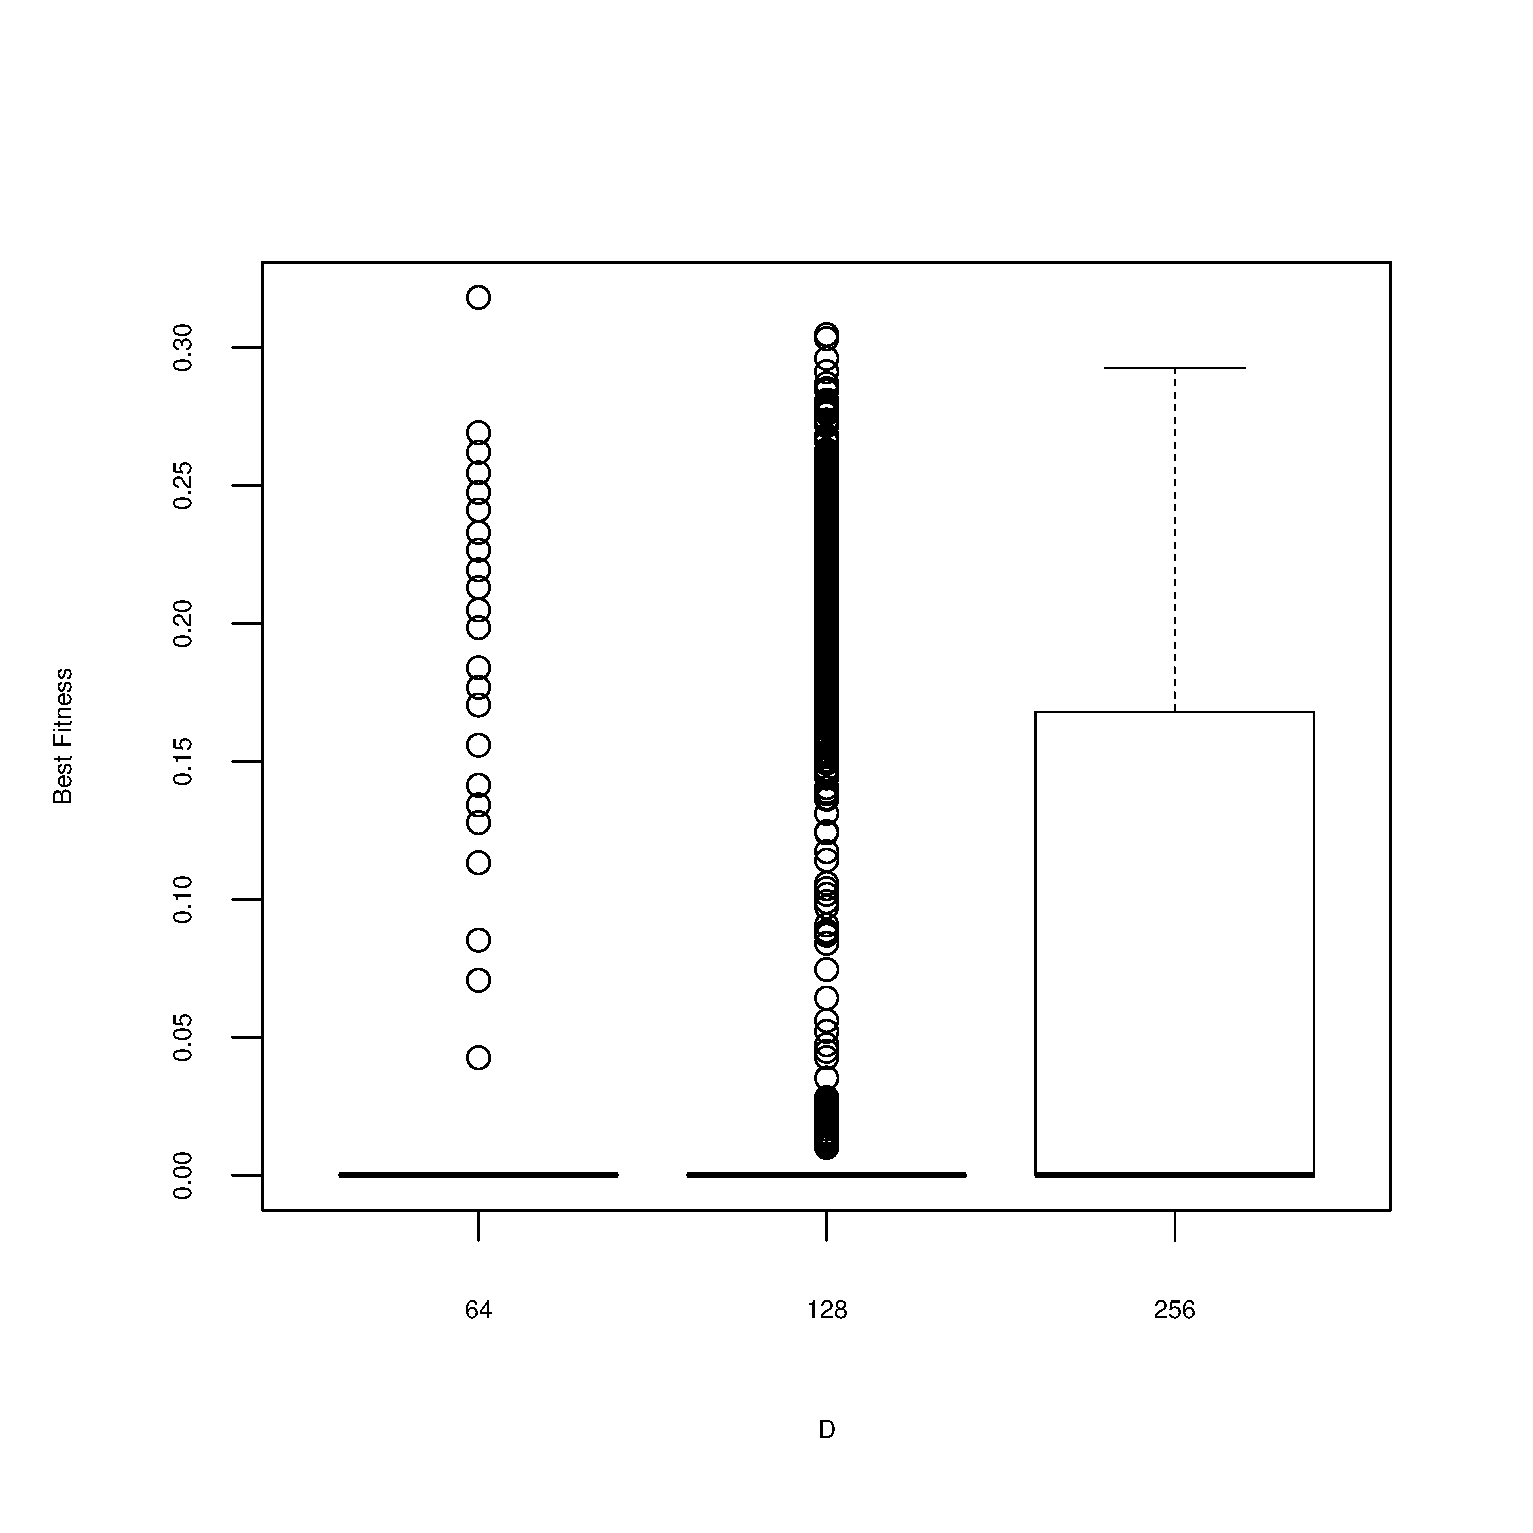
\includegraphics[width=3.7cm]{imags/boxplotz1D.eps}
                \label{fig:e1_d}
        }
        \subfigure[\scriptsize{Scenario 2: Hero}]{
                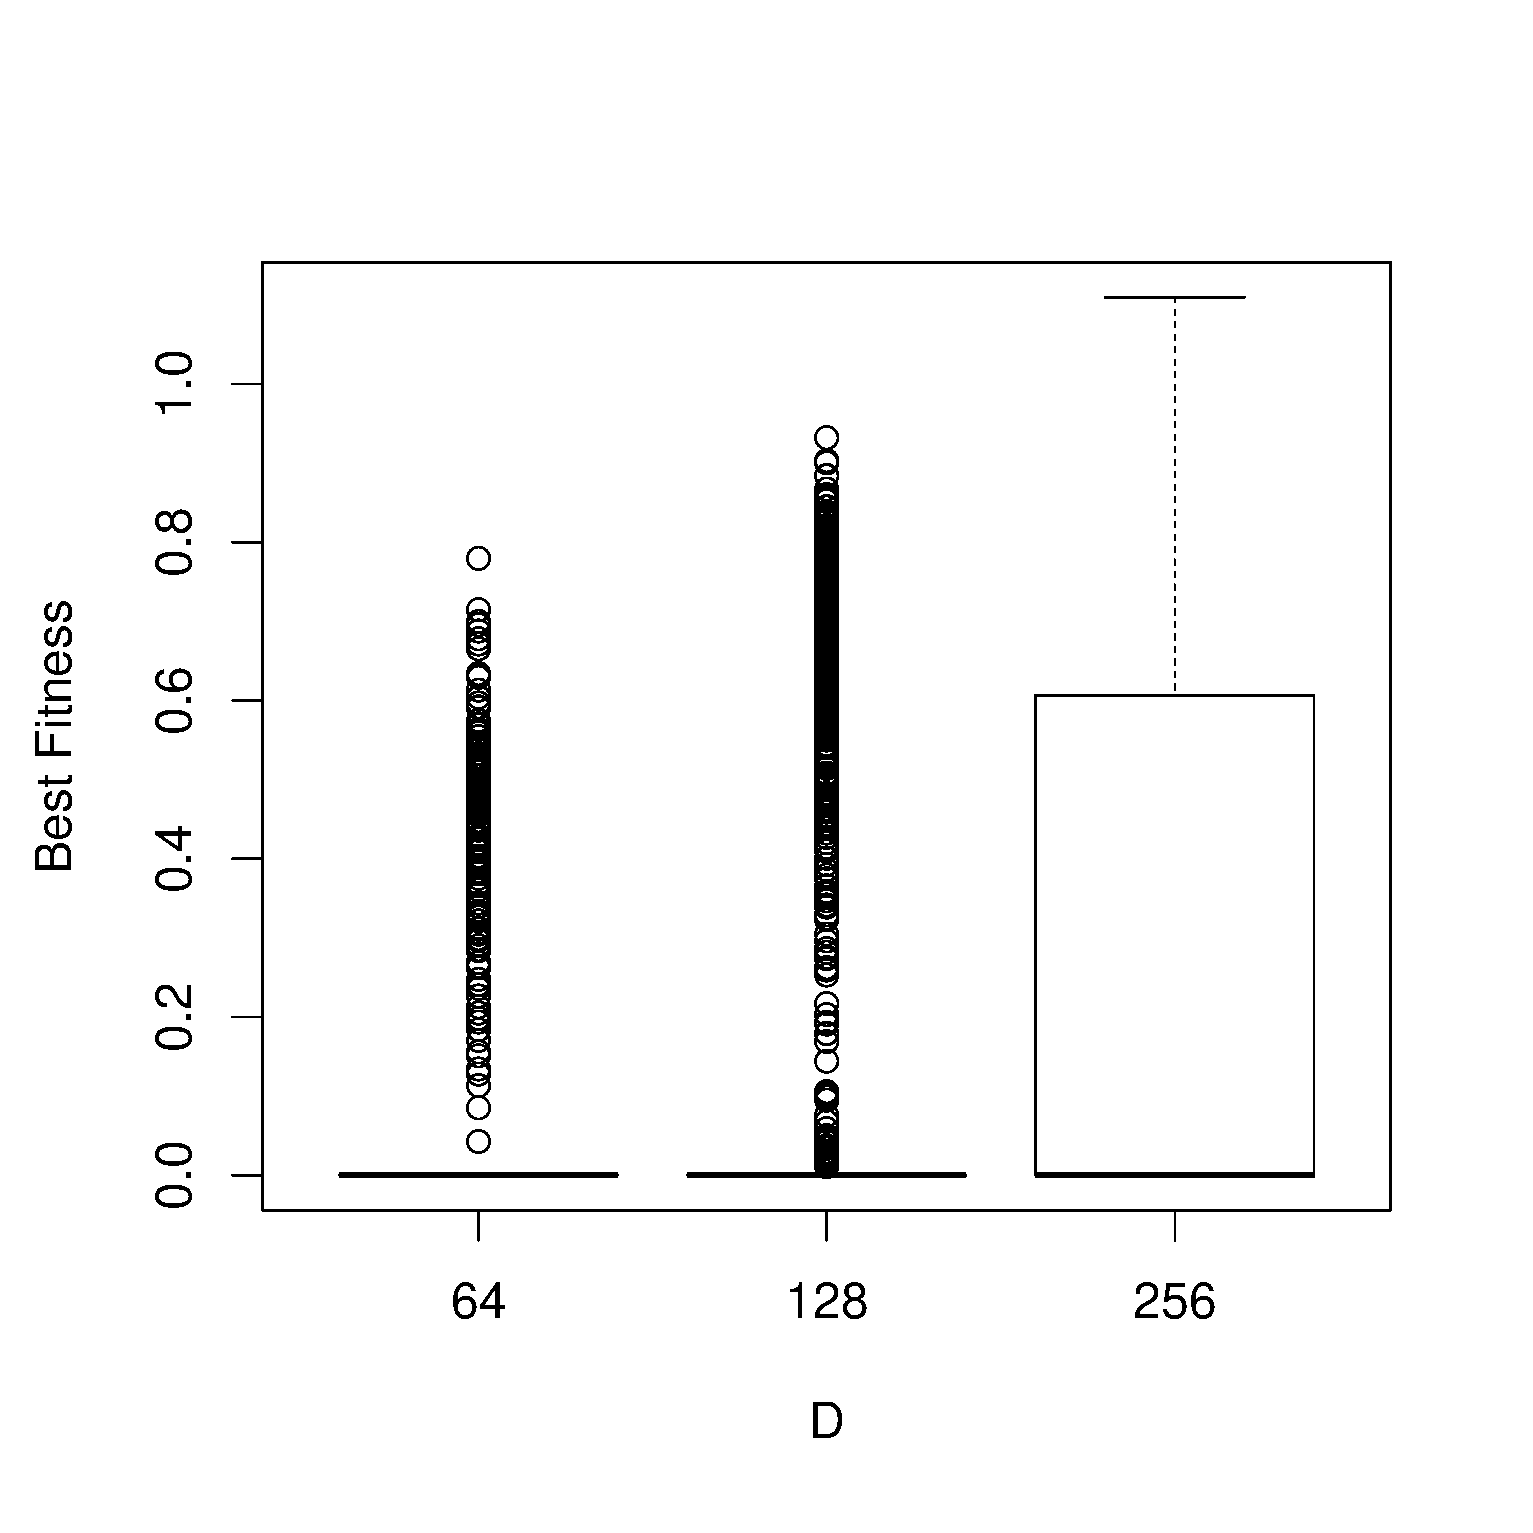
\includegraphics[width=3.7cm]{imags/boxplotz2D.eps}
                \label{fig:e2_d}
        }
        \subfigure[\scriptsize{Scenario 3: Shakespearian}]{
                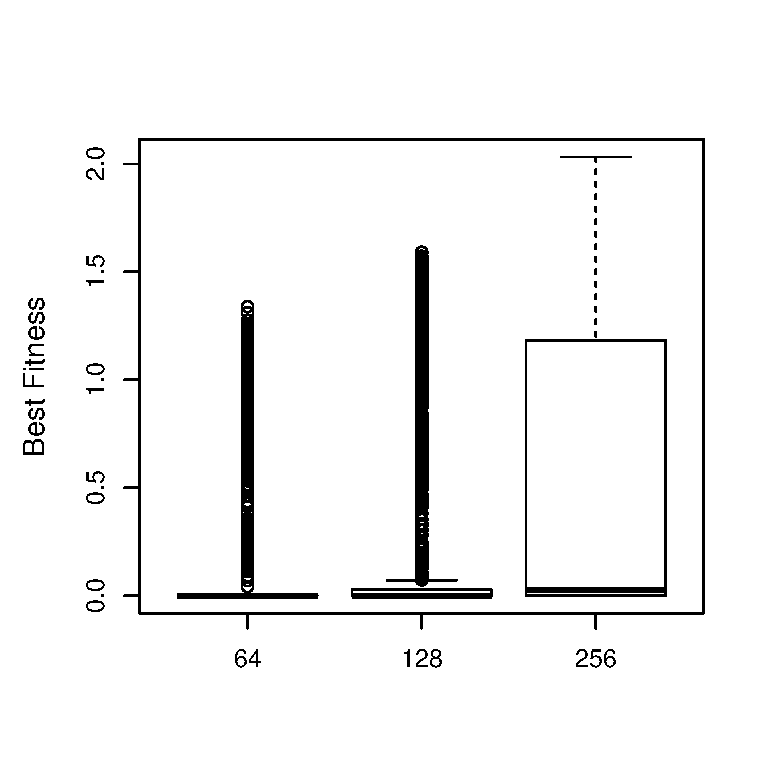
\includegraphics[width=3.7cm]{imags/boxplotz5D.eps}
                \label{fig:e3_d}
        }  
        \caption{Boxplots for parameter D (number of days)}\label{fig:boxplotsD}
\end{figure}

\begin{figure}
        \centering
        \subfigure[\scriptsize{Scenario 1: Villain}]{
                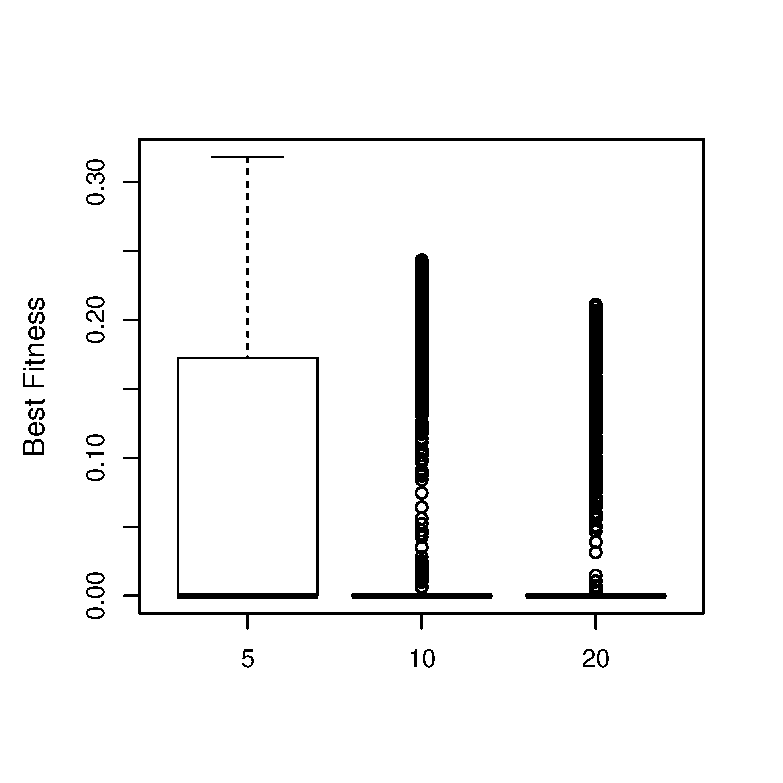
\includegraphics[width=3.7cm]{imags/boxplotz1W.eps}
                \label{fig:e1_w}
        }
        \subfigure[\scriptsize{Scenario 2: Hero}]{
                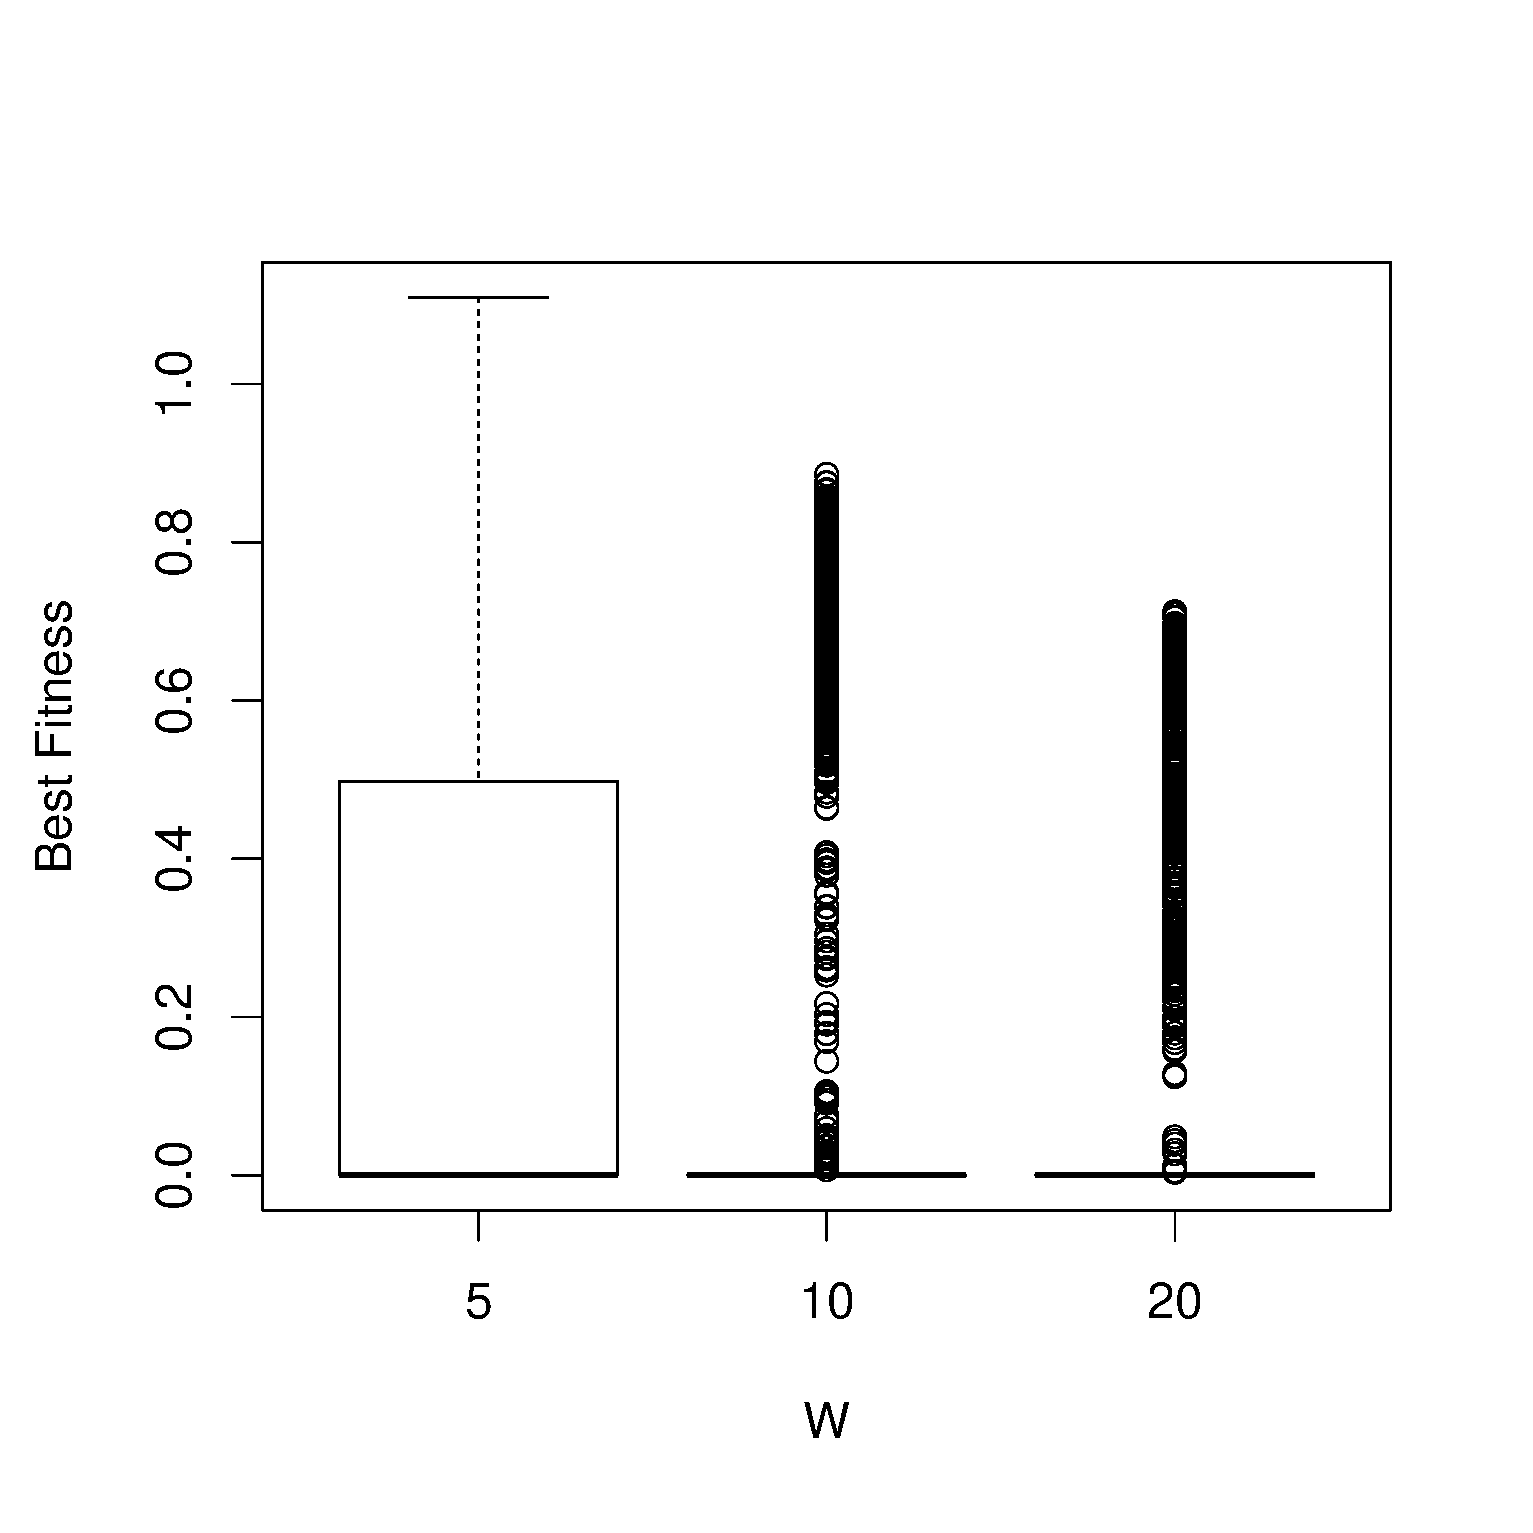
\includegraphics[width=3.7cm]{imags/boxplotz2W.eps}
                \label{fig:e2_w}
        }
        \subfigure[\scriptsize{Scenario 3: Shakespearian}]{
                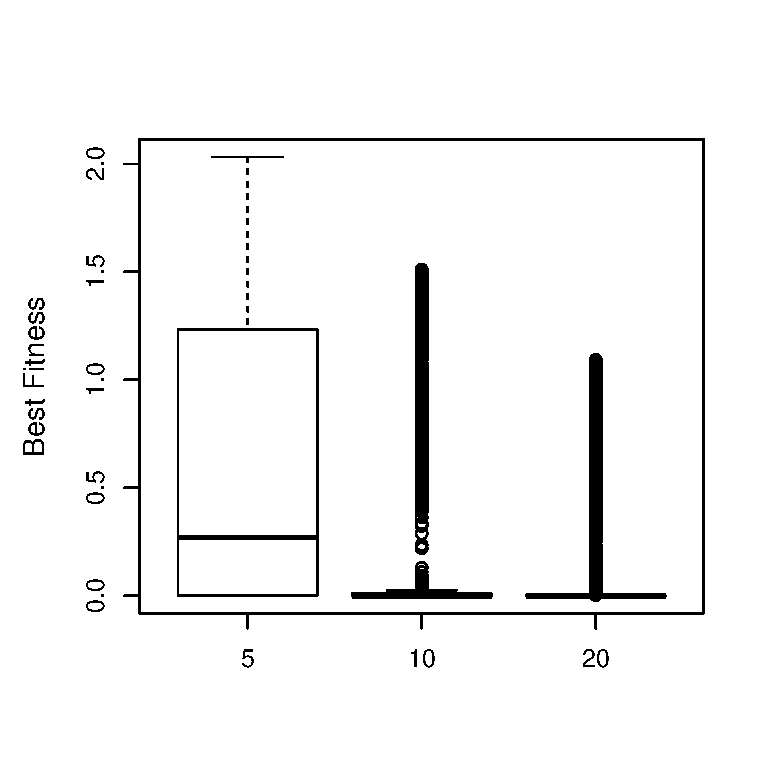
\includegraphics[width=3.7cm]{imags/boxplotz5W.eps}
                \label{fig:e3_w}
        }  
        \caption{Boxplots for parameter W (world size)}\label{fig:boxplotsW}
\end{figure}

\begin{figure}
        \centering
        \subfigure[\scriptsize{Scenario 1: Villain}]{
                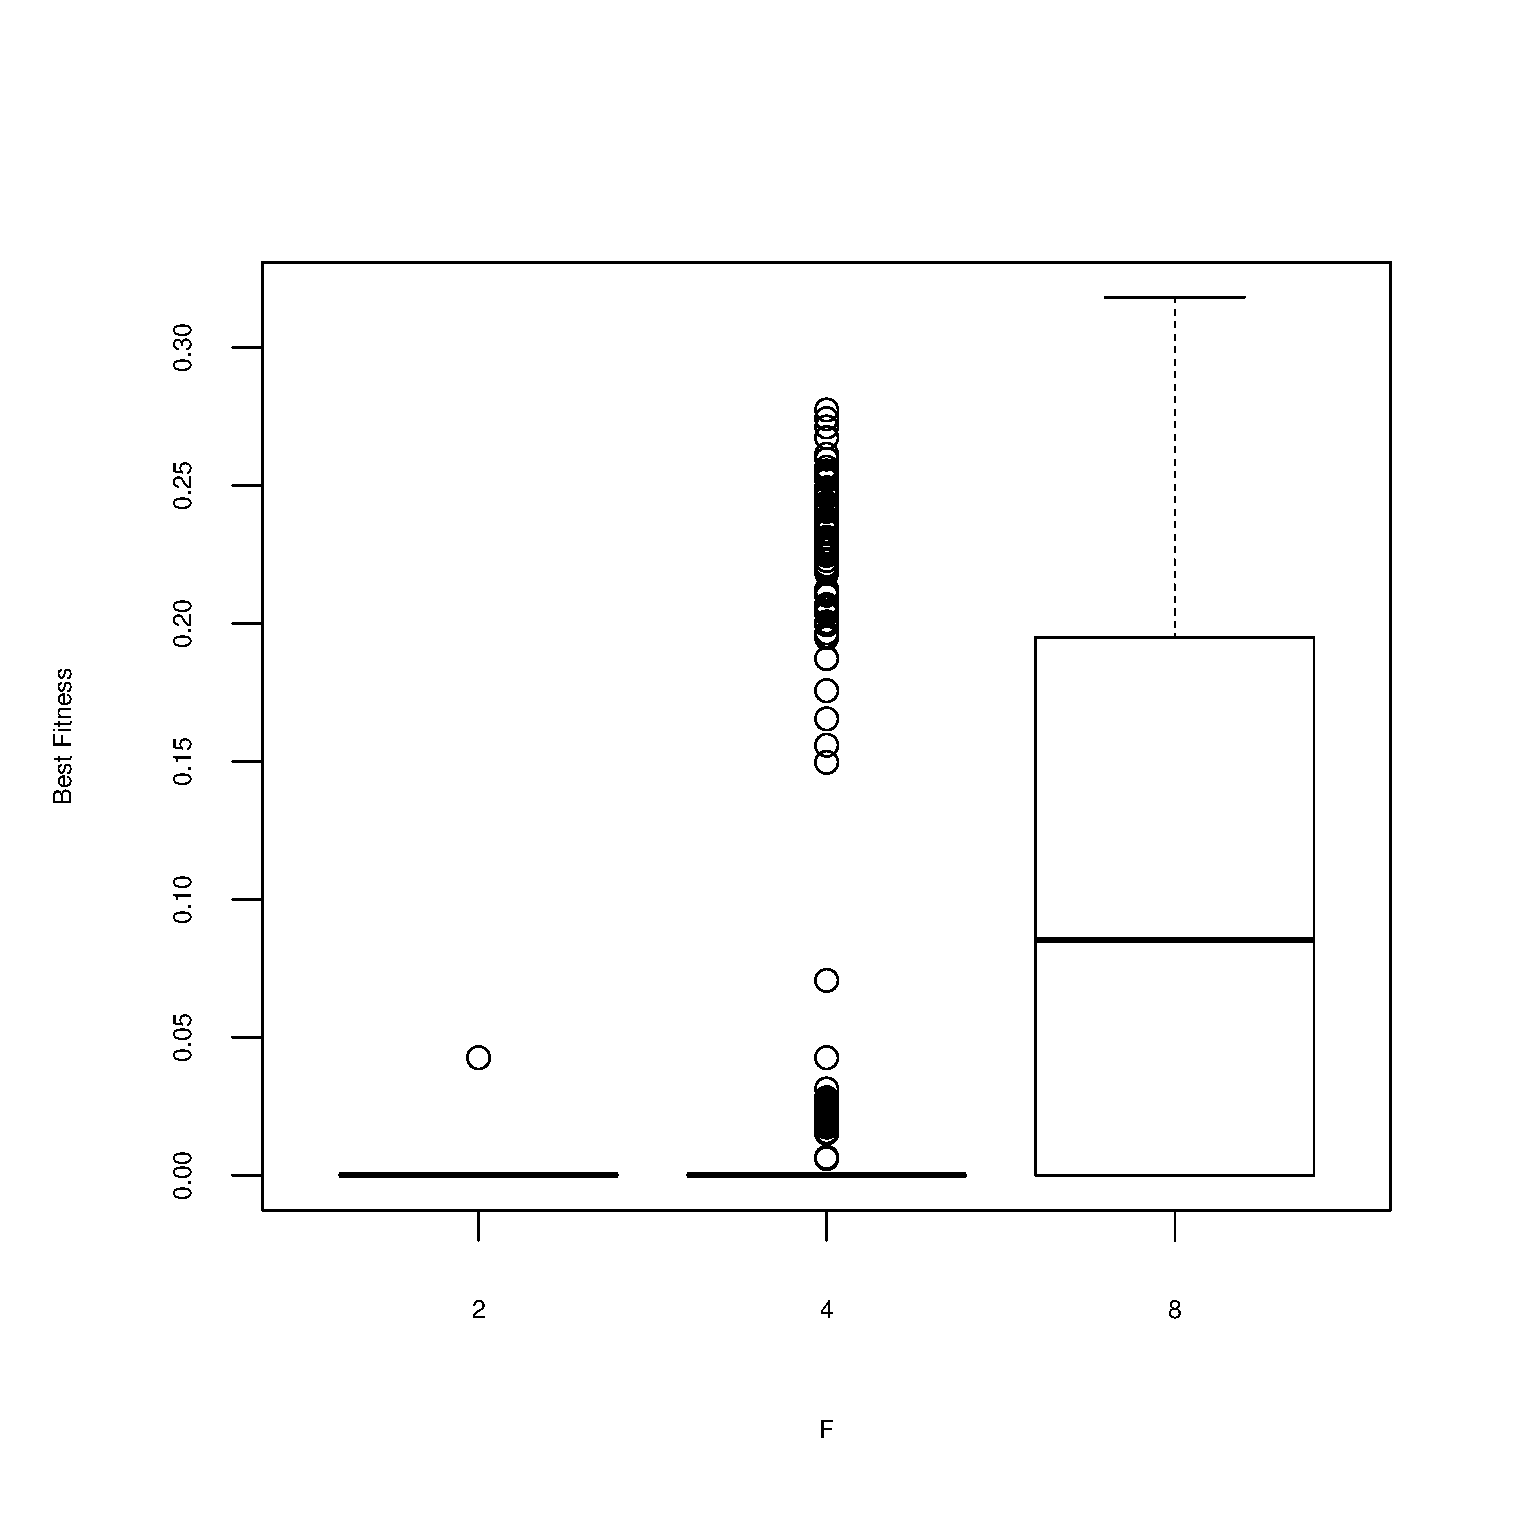
\includegraphics[width=3.7cm]{imags/boxplotz1F.eps}
                \label{fig:e1_f}
        }
        \subfigure[\scriptsize{Scenario 2: Hero}]{
                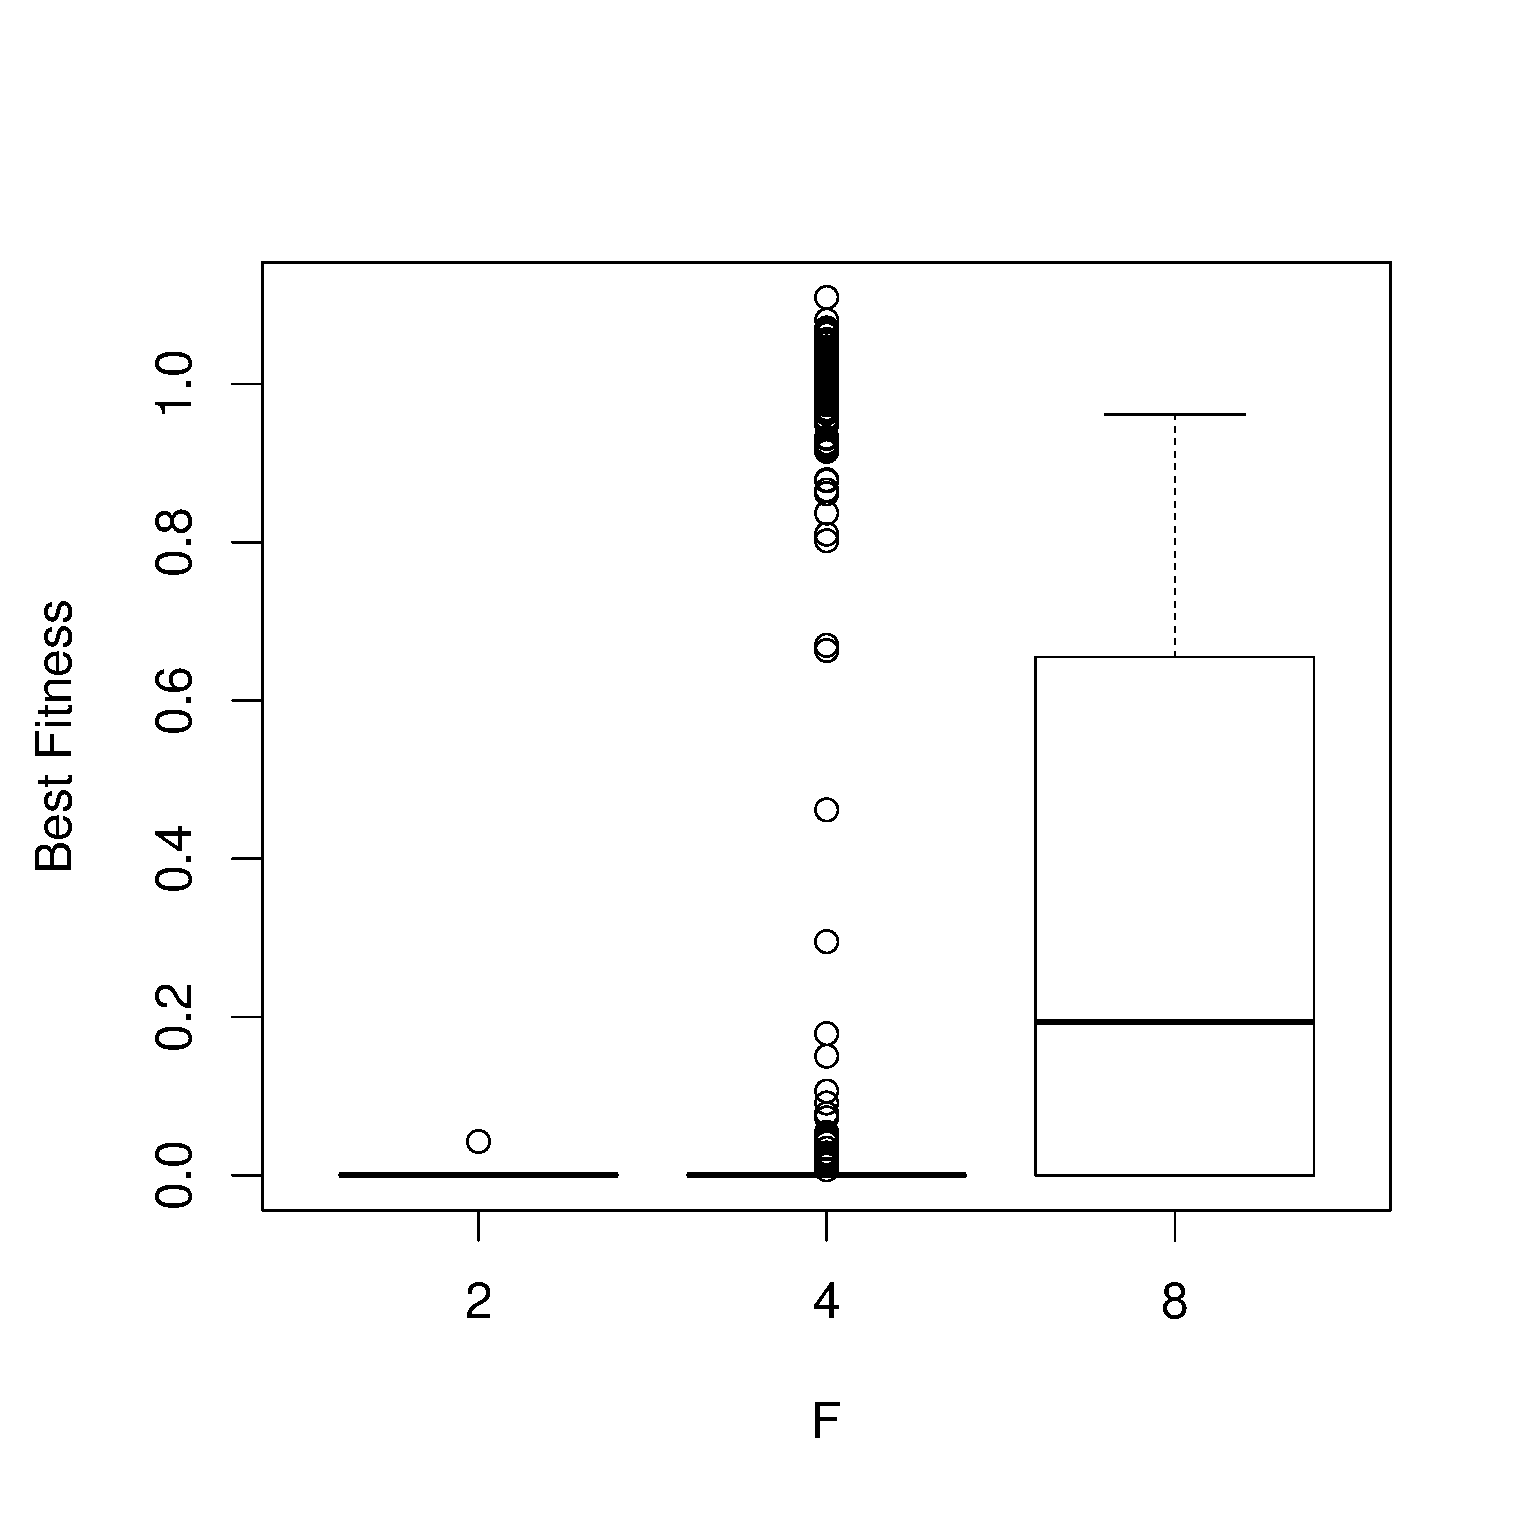
\includegraphics[width=3.7cm]{imags/boxplotz2F.eps}
                \label{fig:e2_f}
        }
        \subfigure[\scriptsize{Scenario 3: Shakespearian}]{
                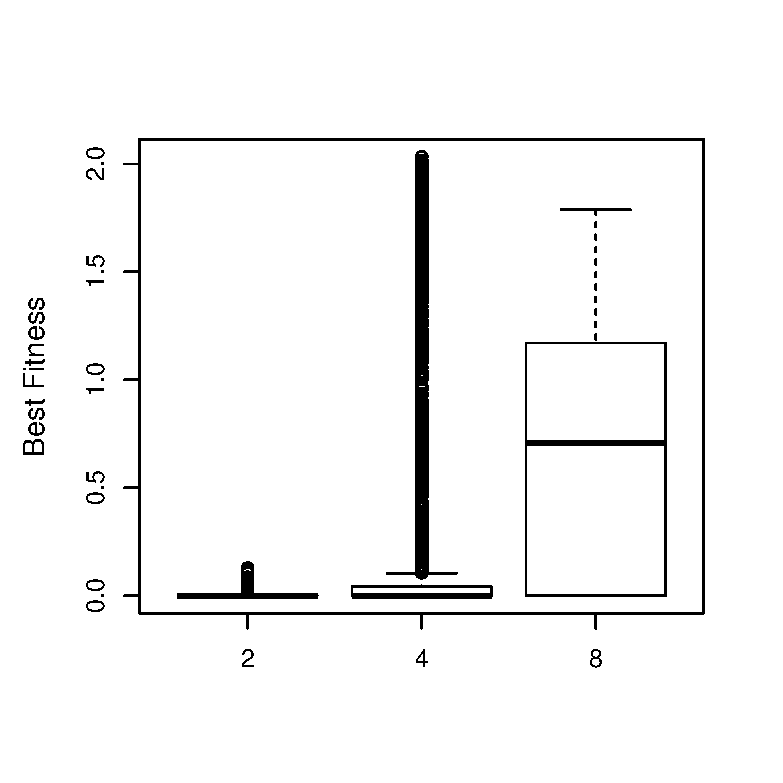
\includegraphics[width=3.7cm]{imags/boxplotz5F.eps}
                \label{fig:e3_f}
        }  
        \caption{Boxplots for parameter F (Food amount)}\label{fig:boxplotsF}
\end{figure}

\begin{figure}
        \centering
        \subfigure[\scriptsize{Scenario 1: Villain}]{
                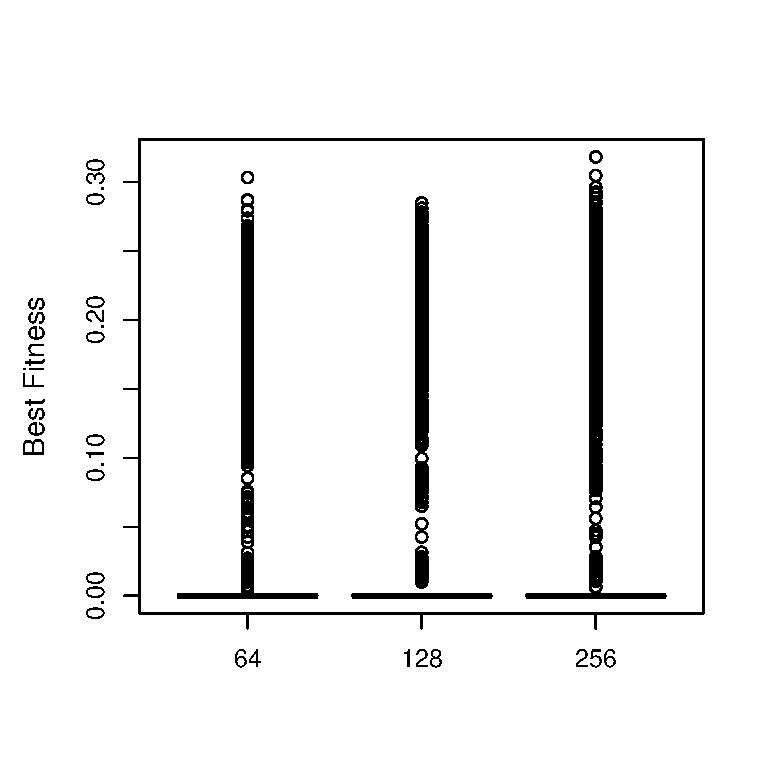
\includegraphics[width=3.7cm]{imags/boxplotz1S.eps}
                \label{fig:e1_s}
        }
        \subfigure[\scriptsize{Scenario 2: Hero}]{
                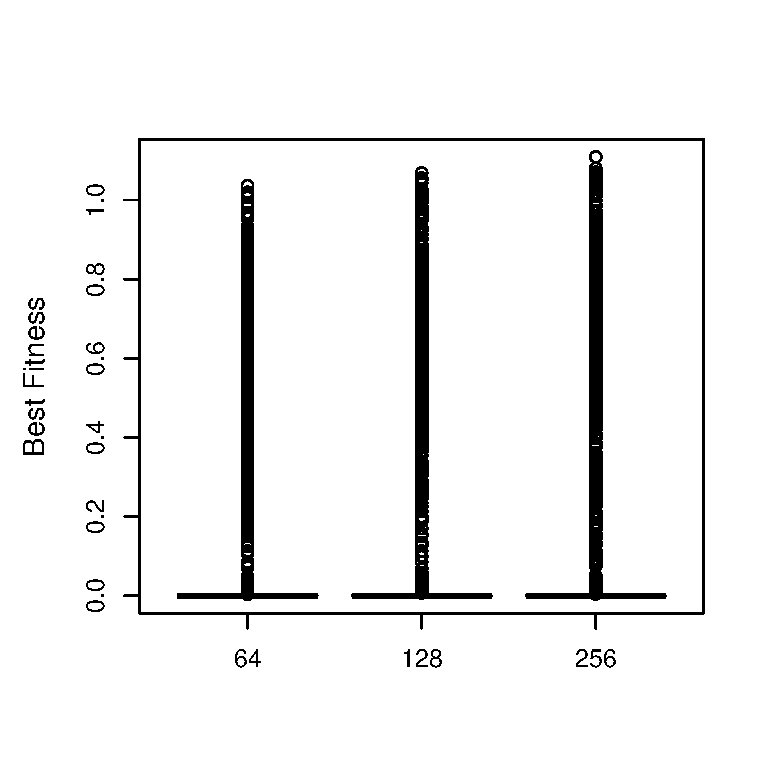
\includegraphics[width=3.7cm]{imags/boxplotz2S.eps}
                \label{fig:e2_s}
        }
        \subfigure[\scriptsize{Scenario 3: Shakespearian}]{
                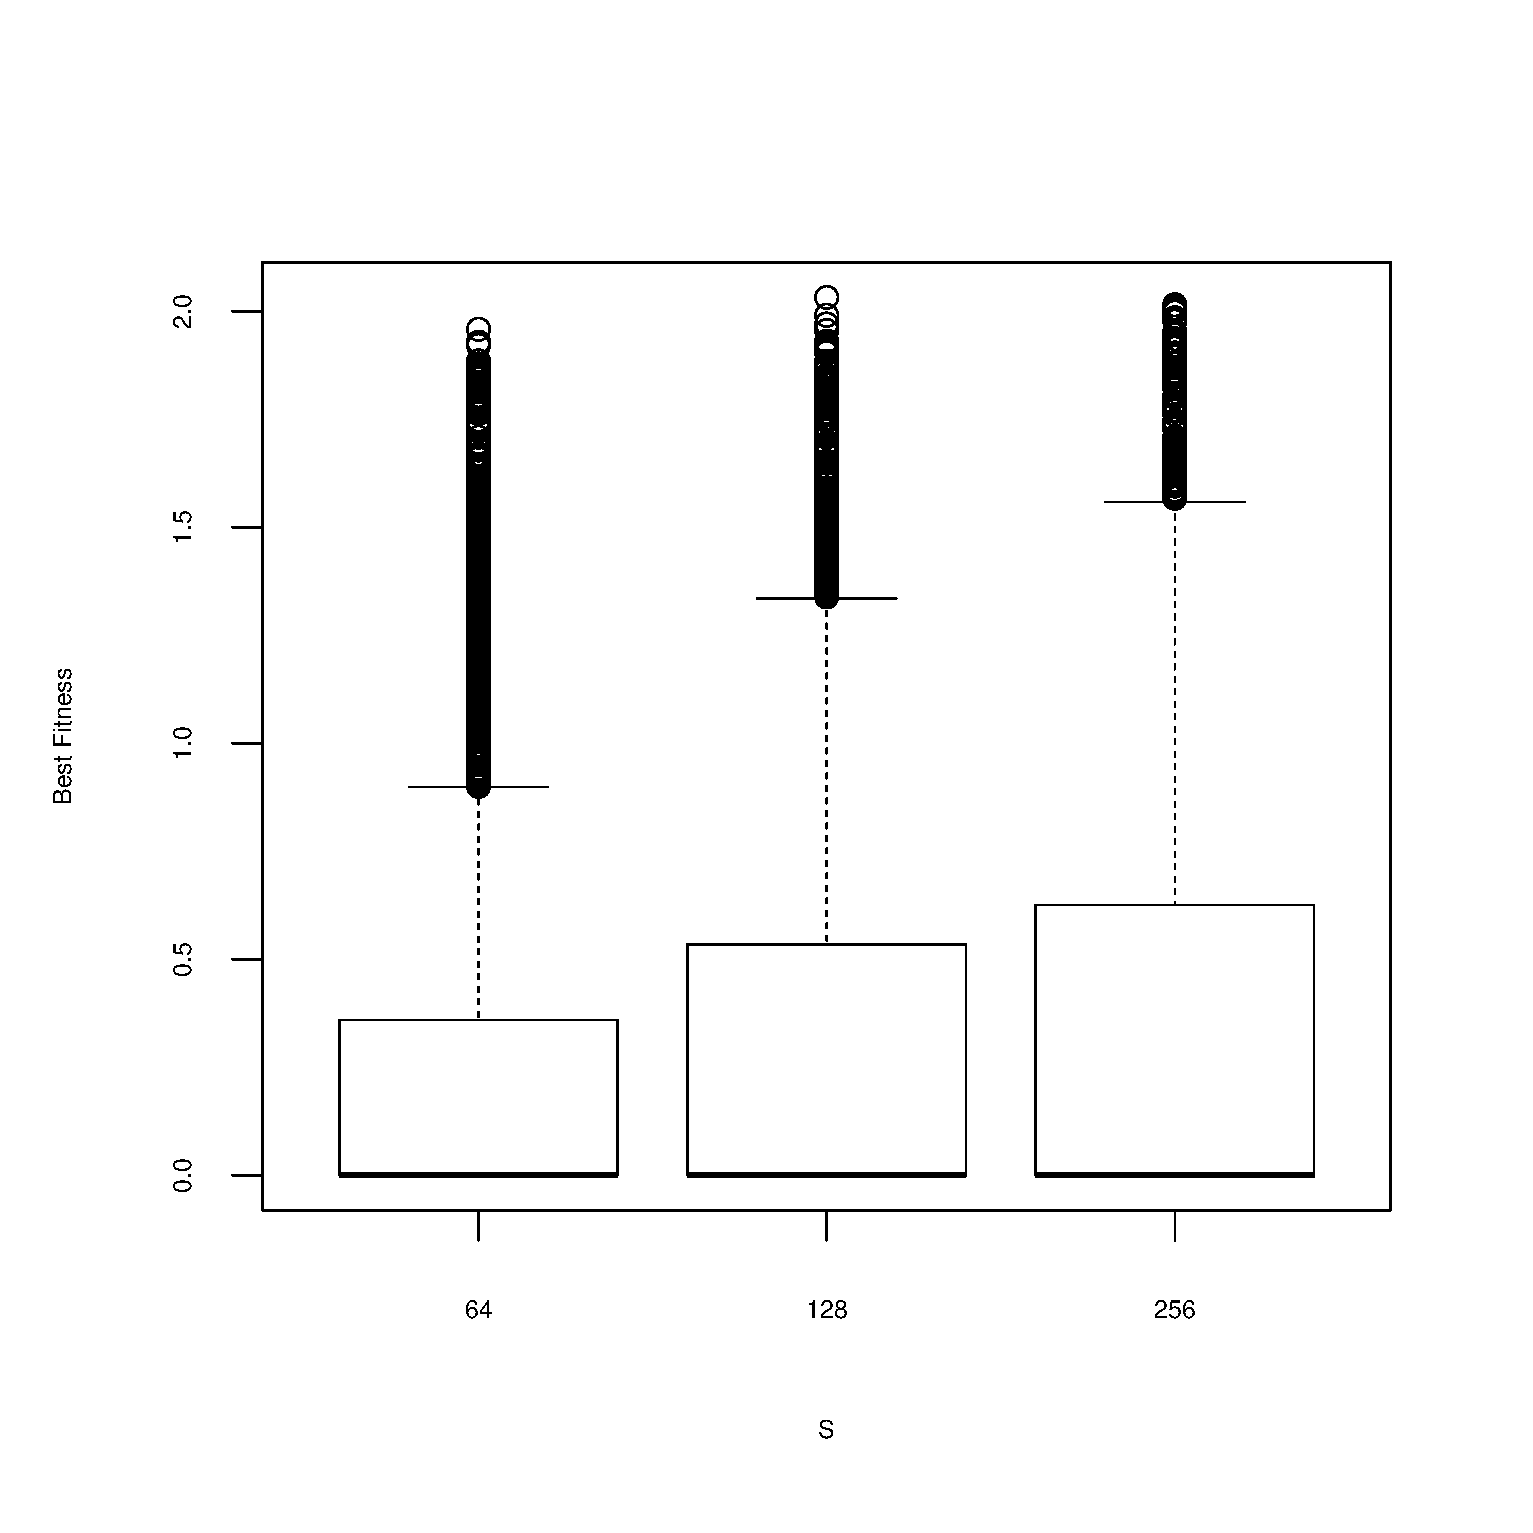
\includegraphics[width=3.7cm]{imags/boxplotz5S.eps}
                \label{fig:e3_s}
        }  
        \caption{Boxplots for parameter S (GA population size)}\label{fig:boxplotsS}
\end{figure}









\section{Conclusions}

\section*{Acknowledgements}

Hidden for double-blind review

\bibliographystyle{unsrt}
\bibliography{geneura,references}

\end{document}
